\documentclass{article}

\usepackage[final, nonatbib]{neurips_2024}

\usepackage[utf8]{inputenc} % allow utf-8 input
\usepackage[T1]{fontenc}    % use 8-bit T1 fonts
%\usepackage{hyperref}       % hyperlinks
%\usepackage{url}            % simple URL typesetting
\usepackage{booktabs}       % professional-quality tables
\usepackage{amsfonts}       % blackboard math symbols
\usepackage{nicefrac}       % compact symbols for 1/2, etc.
\usepackage{microtype}      % microtypography

\usepackage[table,xcdraw]{xcolor} % Add this package for row coloring

\usepackage{url}
\def\UrlBreaks{\do\/\do-}
\usepackage{breakurl}
\usepackage[breaklinks]{hyperref}

\usepackage{amsmath}
\usepackage{graphicx}
\usepackage{threeparttable}
\usepackage{wrapfig}
\usepackage[normalem]{ulem} 
\useunder{\uline}{\ul}{}
\usepackage{placeins}
\usepackage{float}
\usepackage{tikz}
\usetikzlibrary{shapes, arrows.meta, positioning}

\tikzset{
    % Using simpler styles to match the input flowchart's appearance
    process/.style = {rectangle, minimum width=3cm, minimum height=1cm, text centered, draw, text width=3.5cm, align=center, fill=orange!30}, % Adjusted text width
    decision/.style = {diamond, aspect=1.5, minimum width=3cm, minimum height=1cm, text centered, draw, text width=3cm, align=center,  fill=green!30}, % Adjusted text width and aspect ratio
    arrow/.style = {thick,->,>=Stealth}
}

% Define glossex command for Leipzig-style glossing
\newcommand{\glossex}[4]{
  \begin{quote}
  \textbf{#1}: #2\\
  \textit{#3}\\
  `#4'
  \end{quote}
}

% \usepackage{showframe} to debug float placements visually:

\title{Tokens with Meaning: A Hybrid Tokenization Approach for NLP}

\author{
M. Ali Bayram$^1$, Ali Arda Fincan$^2$, Ahmet Semih Gümüş$^2$, Sercan Karakaş$^3$, \\
Banu Diri$^1$, Savaş Yıldırım$^4$, Demircan Çelik$^2$\\
$^1$Yıldız Technical University, $^2$Yeditepe University, $^3$University of Chicago, \\
$^4$Istanbul Bilgi University \\
\texttt{malibayram20@gmail.com}
}

\begin{document}
\maketitle

\begin{abstract}
Tokenization plays a pivotal role in natural language processing (NLP), shaping how textual data is segmented, interpreted, and processed by language models. Despite the success of subword-based tokenization techniques such as Byte Pair Encoding (BPE) and WordPiece, these methods often fall short in morphologically rich and agglutinative languages due to their reliance on statistical frequency rather than linguistic structure. This paper introduces a linguistically informed hybrid tokenization framework that integrates rule-based morphological analysis with statistical subword segmentation to address these limitations. The proposed approach leverages phonological normalization, root-affix dictionaries, and a novel tokenization algorithm that balances morpheme preservation with vocabulary efficiency. It assigns shared identifiers to phonologically variant affixes (e.g., \textit{-ler} and \textit{-lar}) and phonologically altered root forms (e.g., \textit{kitap} vs.\ \textit{kitabı}), significantly reducing redundancy while maintaining semantic integrity. The framework also incorporates special tokens for whitespace and orthographic case, including an \texttt{<uppercase>} token to prevent vocabulary inflation from capitalization. Byte Pair Encoding is integrated to support out-of-vocabulary coverage without compromising morphological coherence. Evaluation on the TR-MMLU benchmark—a large-scale, Turkish-specific NLP benchmark—demonstrates that the proposed tokenizer achieves the highest Turkish Token Percentage (90.29\%) and Pure Token Percentage (85.8\%) among all tested models. Comparative analysis against widely used tokenizers from models such as LLaMA, Gemma, and OpenAI's GPT reveals that the proposed method yields more linguistically meaningful and semantically coherent tokens. A qualitative case study further illustrates improved morpheme segmentation and interpretability in complex Turkish sentences. Although the implementation focuses on Turkish, the underlying methodology is language-independent and adaptable to other languages. This work contributes to ongoing efforts to improve tokenizer design through linguistic alignment, offering a practical and extensible solution for enhancing both interpretability and performance in multilingual NLP systems.

\textbf{Keywords:} Tokenization, Morphologically Rich Languages, Morphological Segmentation, Byte Pair Encoding, Turkish NLP, Linguistic Integrity, Low-Resource Languages
\end{abstract}

\section{Introduction}
Tokenization is the process of mapping raw text into a sequence of discrete units (tokens) that a model can embed and process. It influences vocabulary construction, sequence length, interpretability, and ultimately performance in downstream tasks \cite{liu_roberta_2019}. While subword tokenization has become a standard design choice for transformer-based models, its behavior is not neutral for morphologically rich languages.

Byte Pair Encoding (BPE) \cite{sennrich_neural_2016}, WordPiece \cite{schuster_japanese_2012}, and Unigram \cite{kudo_sentencepiece_2018} address out-of-vocabulary (OOV) words by representing rare forms as compositions of frequent subword units. This improves coverage and keeps vocabularies compact, but it can also split words in ways that cut across morpheme boundaries and blur grammatical function \cite{toraman_impact_2023, kaya_effect_2024}. Such fragmentation is especially relevant for agglutinative languages such as Turkish, where productive suffixation yields many surface forms from relatively few lemmas.

Turkish exhibits rich suffix morphology and systematic morphophonological alternations, including vowel harmony and consonant alternations at morpheme boundaries. For example, suffix allomorphs such as \textit{-lAr} (plural) and \textit{-dAn}/\textit{-tAn} (ablative) realize the same grammatical morpheme under different phonological contexts, and consonant alternations such as \textit{kitap} $\rightarrow$ \textit{kitabı} (p$\rightarrow$b before a vowel) create predictable surface variants of the same stem. Tokenizers that treat these variants as unrelated units can inflate redundancy and reduce the reuse of meaning-bearing units across inflections \cite{bayram_tokenization_2025}.

This paper introduces MFT, a linguistically informed hybrid tokenizer for Turkish. The method combines dictionary-driven morphological segmentation (roots and affixes), a normalization layer that maps common allomorphic variants to shared identifiers, and a controlled subword fallback for open-vocabulary coverage. Roots include a leading space to mark word boundaries, and an orthographic case token preserves capitalization without duplicating vocabulary entries.

We evaluate tokenization quality on TR-MMLU \cite{bayram_setting_2025} using two linguistic alignment metrics: Turkish Token Percentage (TR~\%) and Pure Token Percentage (Pure~\%), which quantify lexical/morphemic coverage and alignment with unambiguous root/affix boundaries, respectively \cite{bayram_tokenization_2025}. To address reviewer concerns about real-world applicability, we further include downstream evaluation on sentence embedding benchmarks. In a controlled random-initialization setting, we compare four matched models (MFT, CosmosGPT2, Mursit, and Tabi) on Semantic Textual Similarity (STS), MTEB-TR, and TurBLiMP, a Turkish benchmark of linguistic minimal pairs \cite{basar_turblimp_2025}.

Our contributions are threefold: we propose a morphology-first hybrid tokenizer for Turkish that is lossless via an explicit decoder; we provide a quantitative and qualitative evaluation of tokenization quality on TR-MMLU against widely used tokenizers; and we report controlled downstream comparisons across four matched embedding models to assess whether improved morpheme alignment translates into better sentence representations.


\section{Related Work}
\label{sec:related_work}

\paragraph{Subword tokenization.}
Subword methods such as BPE \cite{sennrich_neural_2016}, WordPiece \cite{schuster_japanese_2012}, and Unigram-based approaches \cite{kudo_sentencepiece_2018} are widely used because they balance vocabulary size and coverage in neural models \cite{devlin_bert_2019, liu_roberta_2019}. For morphologically rich languages, however, segmentation granularity and vocabulary allocation become more consequential, often leading to higher token ``fertility'' and longer effective sequences \cite{kaya_effect_2024}.

\paragraph{Morphology-aware tokenization for Turkish and beyond.}
Prior work on Turkish shows that tokenizer choice can substantially affect model quality and efficiency. Toraman et al.~\cite{toraman_impact_2023} study tokenization impacts for Turkish language models, while Bayram et al.~\cite{bayram_tokenization_2025} propose linguistic alignment metrics (including TR~\% and Pure~\%) as diagnostics for Turkish tokenization quality. More broadly, morphology-aware segmentation has been explored for tasks such as machine translation \cite{pan_morphological_2020, huck_target_2017} and abstractive summarization \cite{baykara_abstractive_2022}.

\paragraph{Hybrid approaches combining morphology and subwords.}
Hybrid designs that retain linguistic structure while keeping statistical coverage are increasingly common. Jabbar~\cite{jabbar_morphpiece_2024} proposes MorphPiece, which applies morpheme segmentation prior to subword encoding. Asgari et al.~\cite{asgari_morphbpe_2025} propose MorphBPE, a morphology-aware extension of BPE that constrains merges and introduces morphology-based evaluation metrics across multiple languages. Rahimov~\cite{rahimov_milli_2025} introduces miLLi, a dictionary+BPE hybrid for Azerbaijani with a phonological restoration layer that maps allomorphic variants back to canonical roots. Our work aligns with this line but adopts a morphology-first pipeline with explicit allomorph unification and reversible decoding rules.

\paragraph{Turkish-specific baselines and benchmarks.}
Recent Turkish-focused foundation models and benchmarks emphasize the importance of language-specific evaluation and documentation. Türker et al.~\cite{turker_tabibert_2026} introduce TabiBERT and a unified Turkish benchmark, motivating fairer Turkish baselines beyond English-centric tokenizers.
Complementary work on Turkish sentence embeddings highlights practical tokenizer adaptation and evaluation on STS/retrieval benchmarks; Bayram~\cite{bayram_adapting_embeddings_2026} describes token remapping and embedding-alignment techniques for adapting pretrained embedding models to Turkish.

\paragraph{Downstream semantic similarity evaluation.}
Correlation-based evaluation (Pearson/Spearman) is standard for semantic textual similarity, and for agglutinative languages semantic similarity metrics can capture quality beyond surface lexical overlap. Beken Fikri et al.~\cite{beken_fikri_semantic_2021} translate STS resources into Turkish and motivate semantic similarity as an evaluation signal for Turkish text generation and summarization.

\paragraph{Empirical variability.}
Across languages and training setups, the effect of morphology-aware tokenization on downstream model performance can vary. We therefore treat linguistic alignment metrics as interpretable diagnostics for segmentation quality rather than as proof of downstream gains, and we complement them with downstream evaluation (Section~\ref{sec:downstream}).


\section{Methodology}
\label{sec:methodology}

Our tokenizer is designed for morphologically rich, predominantly concatenative systems (e.g., Turkish) where many grammatical functions are expressed through productive suffixation and morphophonological alternations. The key design choice is \emph{morphology-first tokenization}: we prioritize roots and affixes as atomic units when possible, while using subwords only as a fallback for coverage.

\subsection{Resources: Roots, Affixes, and Subwords}
\label{sec:resources}

The tokenizer vocabulary is the union of three components:
\begin{itemize}
  \item \textbf{Root lexicon} (\texttt{kokler.json}): a curated list of Turkish roots and high-frequency lexicalized forms (including selected compounds). Each root may have multiple surface variants mapped to a shared identifier to control vocabulary growth.
  \item \textbf{Affix lexicon} (\texttt{ekler.json}): a curated list of productive suffixes and function markers. Allomorphic variants (e.g., vowel harmony and consonant alternations) are grouped to share identifiers.
  \item \textbf{Subword fallback} (\texttt{bpe\_tokenler.json}): a list of frequent subword units used only when dictionary segmentation fails. In our release, these units are derived from a Turkish subword training run and exported as a lookup table.\footnote{The training corpora include public Turkish corpora hosted on HuggingFace (e.g., \cite{hf_umarigan_turkish_corpus_small, hf_kadirnar_combined_turkish_datasets_v4}).}
\end{itemize}

We additionally include special tokens for whitespace and case handling, notably \texttt{<uppercase>} and an explicit space token.

\paragraph{Identifier ranges and allomorph sets.}
Our released vocabulary uses disjoint identifier ranges for clarity:
(i) roots: ids 0--19999, (ii) affixes: ids 20000--20071, and (iii) subwords: ids 20072--32767.
Importantly, the lexicons map multiple surface strings to shared identifiers to encode allomorph equivalence classes.
In the current release, \texttt{kokler.json} contains 22,231 surface strings mapped to 20,000 root identifiers, and \texttt{ekler.json} contains 177 surface strings mapped to 72 affix identifiers (a direct measure of allomorph unification). The subword fallback consists of 12,696 distinct subword units.

\begin{table}[t]
\centering
\caption{Vocabulary composition in the released Turkish tokenizer. ``Strings'' counts surface forms in JSON files; ``IDs'' counts unique identifiers (i.e., equivalence classes).}
\label{tab:vocab_comp}
\begin{tabular}{lrrr}
\toprule
Component & Strings & IDs & ID range \\
\midrule
Roots (\texttt{kokler.json}) & 22{,}231 & 20{,}000 & 0--19{,}999 \\
Affixes (\texttt{ekler.json}) & 177 & 72 & 20{,}000--20{,}071 \\
Subwords (\texttt{bpe\_tokenler.json}) & 12{,}696 & 12{,}696 & 20{,}072--32{,}767 \\
\bottomrule
\end{tabular}
\end{table}

\subsection{Dictionary Construction and Curation}
\label{sec:dict_construction}

The root lexicon is designed to cover high-frequency lexical material while keeping identifiers stable across surface variants. In practice, this involves (i) collecting high-frequency Turkish word types from large corpora, (ii) filtering and normalizing candidates (e.g., handling Turkish dotted/dotless \textit{i}), and (iii) optionally adding lexicalized multiword compounds as atomic entries when they behave as stable meaning units in the target corpus. This curation improves robustness and interpretability but introduces a key trade-off: the lexicon is language-specific and requires maintenance and domain adaptation.

The affix lexicon encodes productive suffixes and function markers. Each affix identifier can correspond to multiple surface allomorphs. For example, vowel harmony yields alternations over \{a, e\} and \{ı, i, u, ü\}, and consonant hardness can yield alternations such as \textit{d/t} or \textit{k/ğ} (e.g., \textit{kitap} vs.\ \textit{kitabı}; \textit{çocuk} vs.\ \textit{çocuğu}). Instead of treating each surface form as a distinct token, we group them into equivalence classes and select the appropriate surface form at decode time based on phonological context.

\subsection{Normalization and Allomorph Unification}
\label{sec:normalization}

Turkish suffixes and some roots exhibit systematic surface variation driven by vowel harmony and consonant alternations. Our vocabulary therefore supports \emph{many-to-one} mappings: multiple surface strings can map to the same token identifier. During decoding, the appropriate surface allomorph is selected based on phonological context (front/back and rounded/unrounded vowel harmony; consonant hardness).

We explicitly model common Turkish vowel harmony patterns for suffix selection, including alternations over \{a, e\} and \{ı, i, u, ü\}. We also treat \textit{y} as a \emph{vowel or semivowel} in relevant boundary contexts (e.g., buffer consonant behavior), following standard Turkish morphophonology.

\subsection{Encoding Algorithm}
\label{sec:encoding}

The encoder operates by longest-prefix matching against the three vocabularies in a fixed order (roots $\rightarrow$ affixes $\rightarrow$ subwords). It also inserts explicit markers for whitespace and capitalization.

\begin{center}
\fbox{\begin{minipage}{0.96\linewidth}
\textbf{Algorithm 1: Morphology-first hybrid encoding}\\[0.25em]
\textbf{Input:} text string $x$\\
\textbf{Output:} token id sequence $y$\\[0.25em]
1. Split $x$ into whitespace-separated segments; represent spaces explicitly.\\
2. For each segment $w$:
   (a) Split camelCase/PascalCase boundaries (e.g., \texttt{HTTPServer} $\rightarrow$ \texttt{H T T P Server}).\\
   (b) For each subsegment starting with an uppercase letter, emit \texttt{<uppercase>} and lowercase the subsegment.\\
   (c) Scan left-to-right; at each position, emit the longest matching prefix from (roots, then affixes, then subwords).\\
   (d) If no match exists, emit \texttt{<unknown>} and advance by one character.\\
3. Return the concatenated ids.
\end{minipage}}
\end{center}

This procedure is deterministic and designed to be reproducible from the released lookup tables. We use a longest-match heuristic over the \emph{surface form}. This choice improves robustness in practice, but it can diverge from lexical (underlying) analyses in ambiguous cases; we discuss this limitation in Section~\ref{sec:future_work}.

\begin{figure}[H]
\centering
\resizebox{\textwidth}{0.88\textheight}{% Reduced height from full to 88%
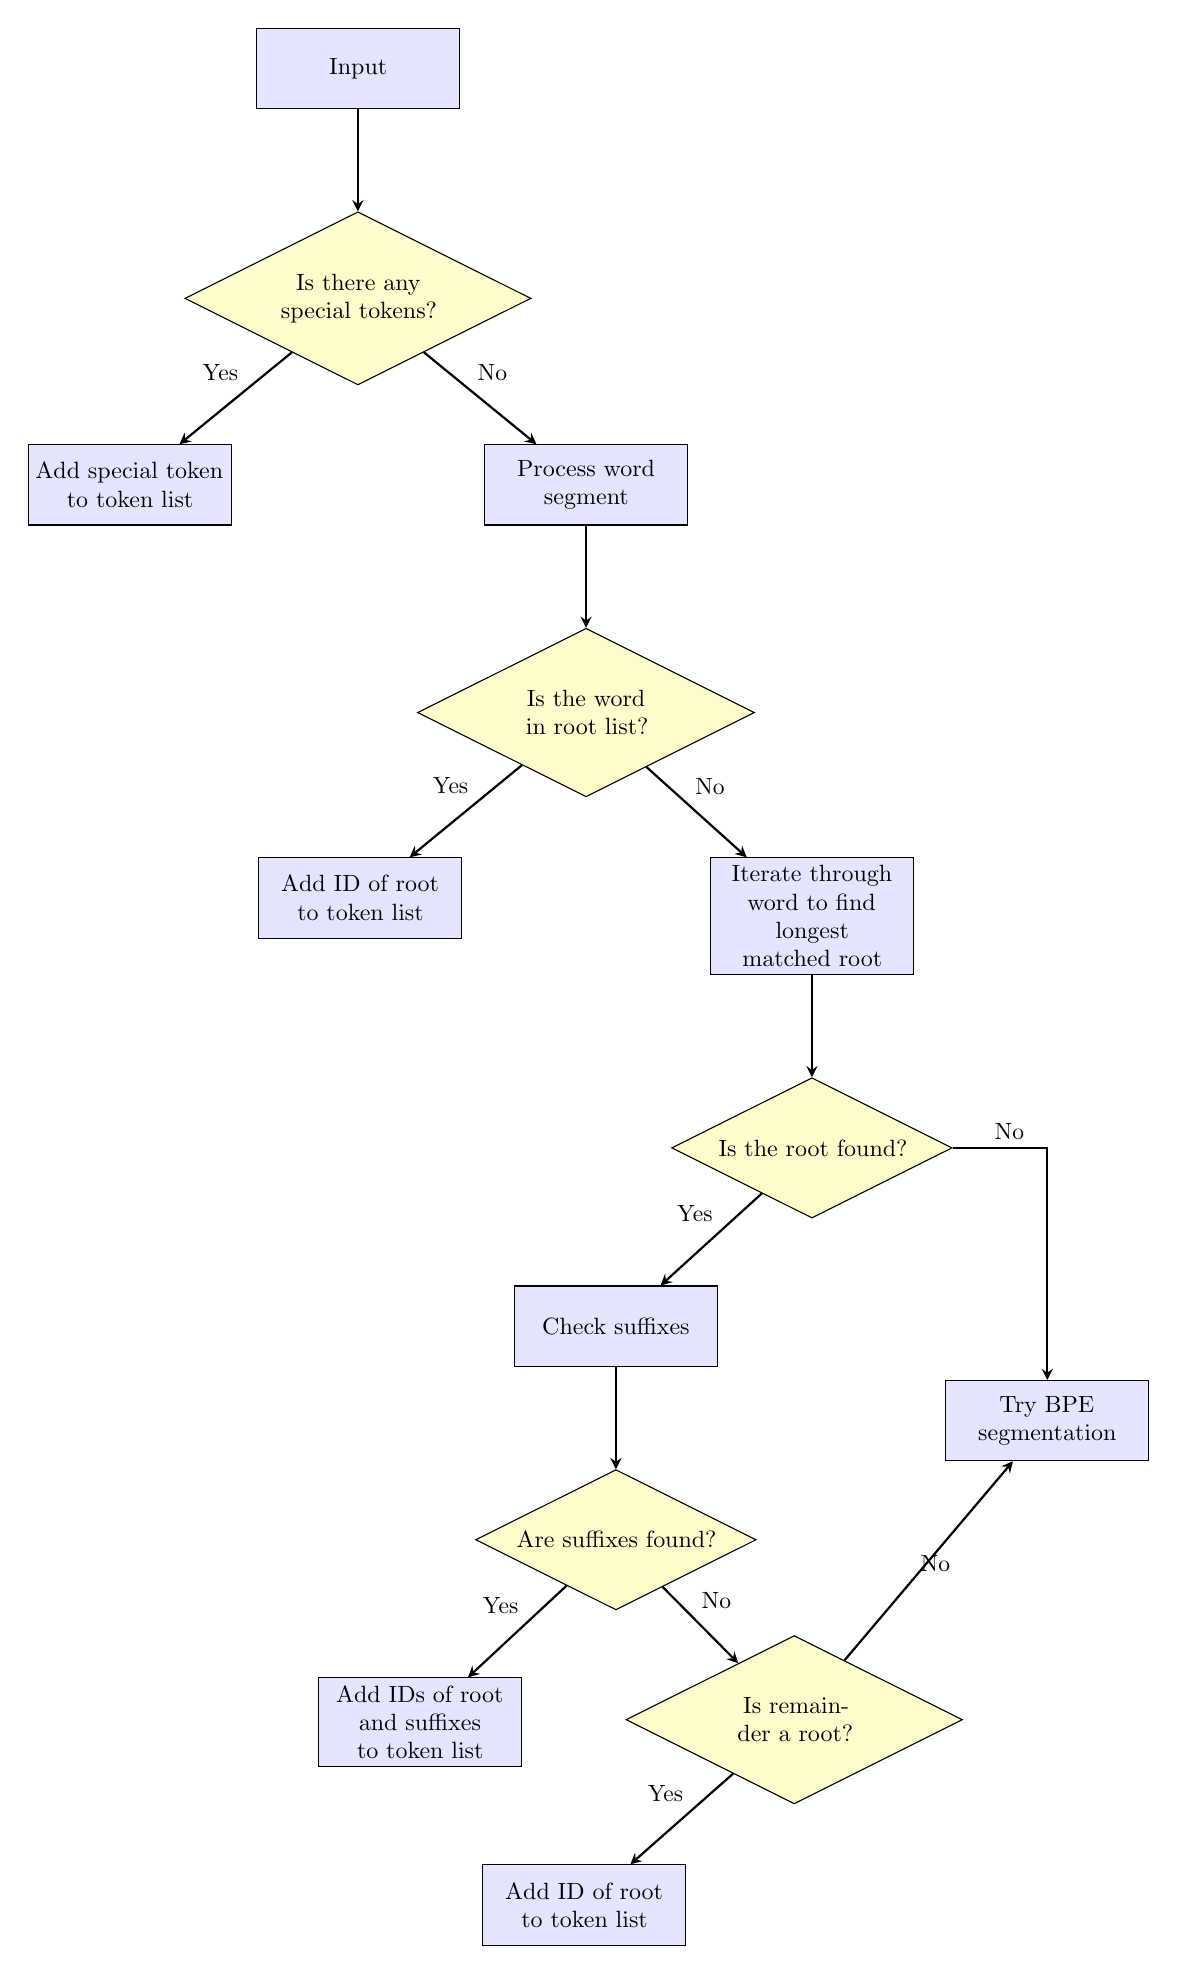
\begin{tikzpicture}[node distance=1.3cm and 1.2cm, every node/.style={transform shape, scale=0.85}]

\tikzstyle{process} = [rectangle, minimum width=2.8cm, text width=2.8cm, minimum height=1.2cm, text centered, draw=black, fill=blue!10]
\tikzstyle{decision} = [diamond, aspect=2, text width=3cm, text centered, draw=black, fill=yellow!20]
\tikzstyle{arrow} = [thick,->,>=stealth]

% Nodes
\node[process] (input_node) {Input};
\node[decision, below=of input_node] (special_check) {Is there any special tokens?};
\node[process, below left=1.3cm and 0.5cm of special_check] (add_special) {Add special token to token list};
\node[process, below right=1.3cm and 0.5cm of special_check] (process_word) {Process word segment};
\node[decision, below=1.3cm of process_word] (root_check) {Is the word in root list?};
\node[process, below left=1.3cm and 0.5cm of root_check] (add_root_id) {Add ID of root to token list};
\node[process, below right=1.3cm and 0.5cm of root_check] (iterate_root) {Iterate through word to find longest matched root};
\node[decision, below=1.3cm of iterate_root] (root_found_check) {Is the root found?};
\node[process, below left=1.3cm and 0.3cm of root_found_check] (check_suffixes) {Check suffixes};
\node[process, below right=2.5cm and 0.8cm of root_found_check] (try_bpe) {Try BPE segmentation};
\node[decision, below=1.3cm of check_suffixes] (suffixes_found_check) {Are suffixes found?};
\node[process, below left=1.3cm and 0.3cm of suffixes_found_check] (add_root_suffix_ids) {Add IDs of root and suffixes to token list};
\node[decision, below right=1.3cm and 0.3cm of suffixes_found_check] (remainder_root_check) {Is remainder a root?};
\node[process, below left=1.3cm and 0.3cm of remainder_root_check] (add_root_id_rem) {Add ID of root to token list};

% Arrows
\draw[arrow] (input_node) -- (special_check);
\draw[arrow] (special_check) -- node[above left, pos=0.4] {Yes} (add_special);
\draw[arrow] (special_check) -- node[above right, pos=0.4] {No} (process_word);
\draw[arrow] (process_word) -- (root_check);
\draw[arrow] (root_check) -- node[above left, pos=0.4] {Yes} (add_root_id);
\draw[arrow] (root_check) -- node[above right, pos=0.4] {No} (iterate_root);
\draw[arrow] (iterate_root) -- (root_found_check);
\draw[arrow] (root_found_check) -- node[above left, pos=0.4] {Yes} (check_suffixes);
\draw[arrow] (root_found_check.east) -| node[above, pos=0.3] {No} (try_bpe.north);
\draw[arrow] (check_suffixes) -- (suffixes_found_check);
\draw[arrow] (suffixes_found_check) -- node[above left, pos=0.4] {Yes} (add_root_suffix_ids);
\draw[arrow] (suffixes_found_check) -- node[above right, pos=0.4] {No} (remainder_root_check);
\draw[arrow] (remainder_root_check) -- node[above left, pos=0.4] {Yes} (add_root_id_rem);
\draw[arrow] (remainder_root_check) -- node[above right, pos=0.4] {No} (try_bpe);

\end{tikzpicture}%
}
\caption{Tokenization decision flow with root, suffix, and fallback segmentation logic.}
\label{fig:decision_flow}
\end{figure}

\subsection{Decoding and Surface Form Reconstruction}
\label{sec:decoding}

Decoding maps token identifiers back to text using reverse vocabularies and morphophonological rules. If an id corresponds to an allomorph set (multiple surface strings), the decoder selects the surface form based on the preceding lexical material (vowel harmony; consonant hardness). For the \texttt{<uppercase>} marker, the decoder capitalizes the subsequent token.

This design enables near-lossless reconstruction for typical Turkish text where unknown tokens are rare and capitalization is mostly word-initial. However, full losslessness is not guaranteed: unknown tokens are rendered as placeholders, and sequences of all-caps letters (e.g., acronyms) may be imperfectly reconstructed under the current marker design. We treat this as an explicit edge case for future refinement.

\paragraph{Decoder rules (implementation summary).}
Our public decoder (\texttt{turkish\_decoder.py}) implements rule-based selection for affix allomorphs based on the most recent vowel in the preceding token (front/back; rounded/unrounded) and the hardness of the final consonant (e.g., \textit{d/t} alternations). In addition, a small set of root identifiers are associated with multiple surface root forms (e.g., variants triggered by vowel-initial suffixes), and the decoder selects among them based on whether the next token begins with a vowel. These rules are intentionally lightweight: they do not attempt full morphological disambiguation, and they operate on local context rather than syntactic structure.

\paragraph{Complexity.}
The encoder performs longest-prefix matching over bounded prefix lengths, making runtime approximately linear in input length with a constant factor determined by maximum token string lengths in each lexicon. In practice, this enables efficient tokenization while preserving the transparency of a rule-based pipeline.

\subsection{Worked Example with Leipzig-Style Glossing}
\label{sec:glossing}

We illustrate morphology-first segmentation on a multi-morpheme Turkish word:

\glossex{Example 1}{anla-yabil-dik-ler-imiz-den}{understand-\textsc{abil}-\textsc{nmlz}-\textsc{pl}-\textsc{1pl.poss}-\textsc{abl}}{``from what we were able to understand''}

This example highlights two goals: (i) preserve the root as a stable unit, and (ii) isolate productive suffixes so that grammatical meaning is represented compositionally rather than through arbitrary subword fragments.
We follow standard Leipzig-style conventions for interlinear glossing \cite{leipzig_glossing_rules}.

\begin{figure}[H]
\centering
\resizebox{\textwidth}{!}{%
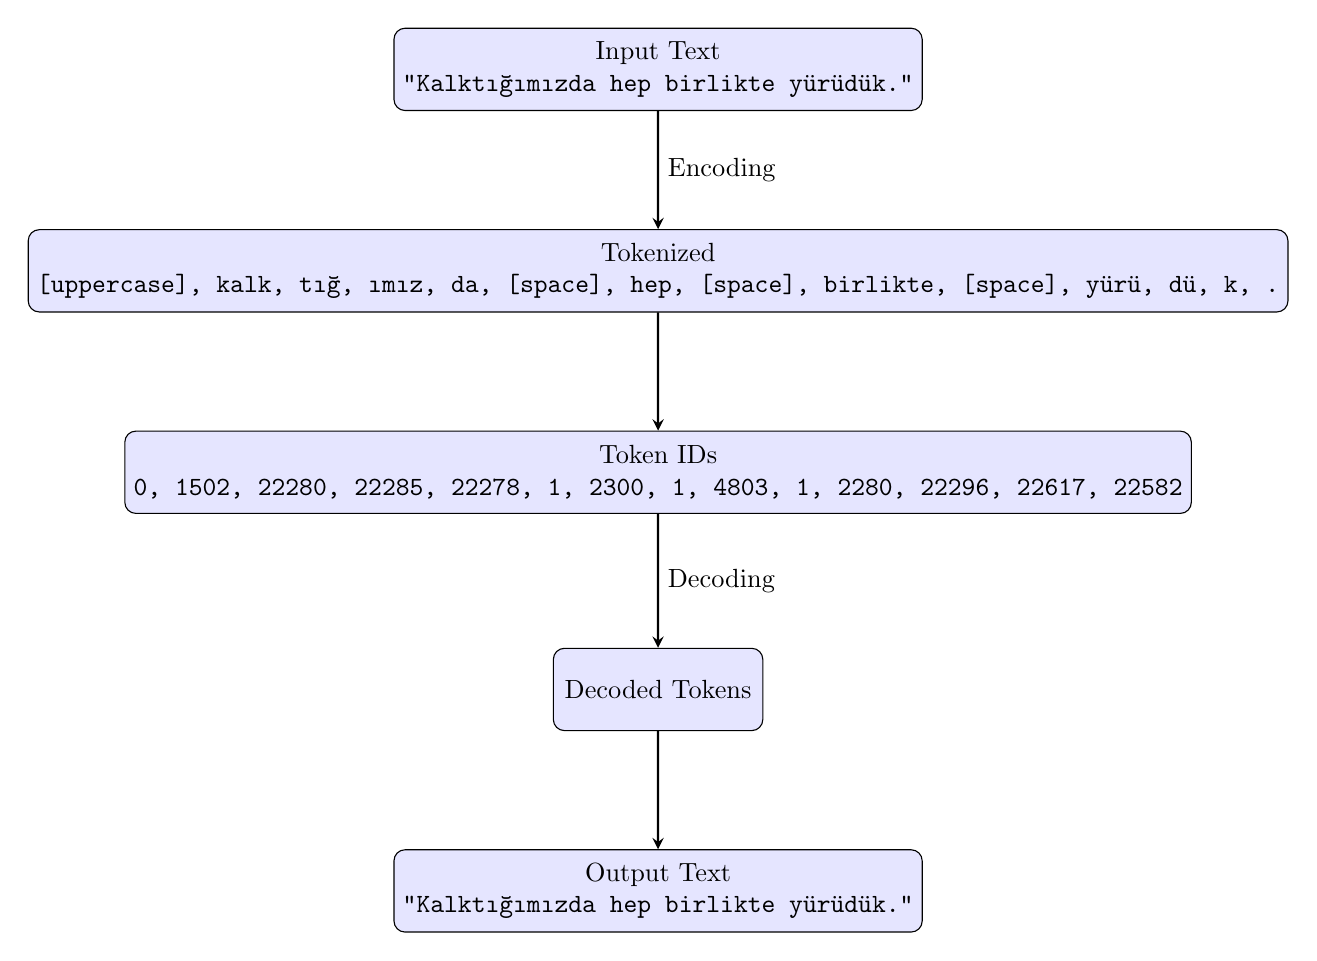
\begin{tikzpicture}[node distance=1.5cm and 0.7cm, every node/.style={transform shape, scale=0.95}]
\tikzset{
  mystep/.style={
    rectangle, rounded corners, draw=black, fill=blue!10,
    minimum height=1.1cm, minimum width=2.8cm,
    text centered, align=center
  },
  arrow/.style={->, thick, >=stealth}
}

\node[mystep] (text) {Input Text \\ \texttt{"Kalktığımızda hep birlikte yürüdük."}};
\node[mystep, below=of text] (tokenized) {Tokenized \\ \texttt{[uppercase], kalk, tığ, ımız, da, [space], hep, [space], birlikte, [space], yürü, dü, k, .}};
\node[mystep, below=of tokenized] (ids) {Token IDs \\ \texttt{0, 1502, 22280, 22285, 22278, 1, 2300, 1, 4803, 1, 2280, 22296, 22617, 22582}};
\node[mystep, below=1.7cm of ids] (reconstruct) {Decoded Tokens};
\node[mystep, below=of reconstruct] (finaltext) {Output Text \\ \texttt{"Kalktığımızda hep birlikte yürüdük."}};

\draw[arrow] (text) -- (tokenized) node[midway, right] {Encoding};
\draw[arrow] (tokenized) -- (ids);
\draw[arrow] (ids) -- (reconstruct) node[midway, right] {Decoding};
\draw[arrow] (reconstruct) -- (finaltext);

\end{tikzpicture}%
}
\caption{Encoding and decoding process for the sentence “Kalktığımızda hep birlikte yürüdük.”}
\label{fig:encoding_process}
\end{figure}


\section{Results and Analysis}
\label{sec:results}

\subsection{Metrics: TR\% and Pure\%}
\label{sec:metrics}

We report two linguistic alignment metrics introduced in \cite{bayram_tokenization_2025}. Let a tokenizer produce a token sequence $t_1,\dots,t_N$ for a corpus. TR~\% measures how many produced tokens correspond to Turkish lexical or morphemic units under a Turkish lexical resource:
\[
\mathrm{TR\%} = \frac{\sum_{i=1}^N \mathbb{1}[\mathrm{TurkishUnit}(t_i)]}{N}\times 100.
\]
Pure~\% measures how many produced tokens align with unambiguous root/affix boundaries:
\[
\mathrm{Pure\%} = \frac{\sum_{i=1}^N \mathbb{1}[\mathrm{PureUnit}(t_i)]}{N}\times 100.
\]
In our implementation, \texttt{turkish\_tokenizer} uses explicit root and affix vocabularies, so the set of ``TurkishUnit'' and ``PureUnit'' tokens is defined directly by these lexicons. For baseline tokenizers, these metrics are computed via the same evaluation pipeline from \cite{bayram_tokenization_2025}. While TR~\% and Pure~\% are interpretable diagnostics for segmentation quality, we complement them with downstream task evaluation in Section~\ref{sec:downstream}.

\subsection{Tokenization quality on TR-MMLU}
\label{sec:trmmlu}

The performance of the proposed morphological tokenizer was evaluated using the TR-MMLU benchmark dataset, which comprises over 1.6 million characters and approximately 200,000 words curated specifically for Turkish \cite{bayram_setting_2025}. This dataset is designed to reflect the linguistic complexity of Turkish, including its rich morphology, agglutinative structures, and diverse syntactic constructions. As such, it provides a rigorous basis for assessing tokenization quality in morphologically complex languages.

The evaluation compared five different tokenizers: \texttt{google/gemma-2-9b}, \texttt{meta-llama/Llama-3.2-3B}, \texttt{Qwen/Qwen2.5-7B-Instruct}, \texttt{CohereForAI/aya-expanse-8b}, and the proposed \texttt{turkish\_tokenizer}. Each tokenizer was assessed using a consistent set of linguistic and computational metrics introduced in \cite{bayram_tokenization_2025}. These metrics include total token count, vocabulary size, number of unique tokens, Turkish Token Percentage (TR~\%), and Pure Token Percentage (Pure~\%). TR~\% quantifies the proportion of tokens that correspond to valid Turkish words or morphemes, while Pure~\% measures the proportion of tokens that fully align with unambiguous root or affix boundaries, thus reflecting morphological integrity.

\begin{table}[h]
\centering
\caption{Performance of the proposed \texttt{turkish\_tokenizer} on the TR-MMLU dataset.}
\label{tab:turkish_tokenizer_results}
\begin{tabular}{|l|c|}
\hline
\rowcolor[HTML]{DDDDDD} 
\textbf{Metric} & \textbf{Value} \\ \hline
Vocabulary Size & 32,768 \\ \hline
Total Token Count & 707,727 \\ \hline
Processing Time (s) & 0.6714 \\ \hline
Unique Token Count & 11,144 \\ \hline
Turkish Token Count & 10,062 \\ \hline
Turkish Token Percentage (TR \%) & 90.29\% \\ \hline
Pure Token Count & 9,562 \\ \hline
Pure Token Percentage (Pure \%) & 85.80\% \\ \hline
\end{tabular}
\end{table}

\begin{table}[h]
\centering
\caption{Linguistic alignment comparison on TR-MMLU. We report TR~\% and Pure~\% for tokenizers where the corresponding metric was computed in our evaluation pipeline; missing entries indicate the metric was not computed in this run.}
\label{tab:alignment_comparison}
\begin{tabular}{lcc}
\toprule
Tokenizer & TR (\%) & Pure (\%) \\
\midrule
turkish\_tokenizer (ours) & \textbf{90.29} & \textbf{85.80} \\
google/gemma-2-9b & 40.96 & 28.49 \\
meta-llama/Llama-3.2-3B & 45.77 & 31.45 \\
Qwen/Qwen2.5-7B-Instruct & 40.39 & -- \\
CohereForAI/aya-expanse-8b & 53.48 & -- \\
\bottomrule
\end{tabular}
\end{table}

The proposed \texttt{turkish\_tokenizer} demonstrated the highest linguistic alignment across all evaluated metrics. It achieved a TR~\% of 90.29\% and a Pure~\% of 85.80\%, substantially outperforming all competing tokenizers. In comparison, \texttt{google/gemma-2-9b} reached a TR~\% of only 40.96\% and a Pure~\% of 28.49\%, indicating that the majority of its tokens do not represent full morphemes. Similarly, \texttt{meta-llama/Llama-3.2-3B} produced a TR~\% of 45.77\% and a Pure~\% of 31.45\%, while \texttt{Qwen2.5} and \texttt{aya-expanse} achieved TR~\% values of 40.39\% and 53.48\%, respectively.

Despite employing significantly smaller vocabulary sizes, the proposed tokenizer demonstrated better linguistic segmentation. With a vocabulary of 32,768 tokens and 11,144 unique tokens used during evaluation, it balanced generalization and expressiveness more effectively than models such as \texttt{gemma-2-9b} and \texttt{aya-expanse}, which rely on vocabularies of over 255,000 tokens. These large-vocabulary tokenizers, rooted in frequency-based subword segmentation, tend to fragment morphologically rich expressions and introduce ambiguity in downstream tasks. In contrast, the morphological awareness of the \texttt{turkish\_tokenizer} enables semantically coherent token formation and more consistent syntactic parsing.

Although the total token count generated by the proposed tokenizer (707,727) exceeds those of the other models—for instance, \texttt{aya-expanse} produced 434,526 tokens—this increase is offset by gains in interpretability and linguistic fidelity. High TR~\% and Pure~\% scores suggest reduced reliance on spurious subword splits and improved preservation of morphosyntactic structure. This is particularly beneficial for tasks such as syntactic parsing, translation, summarization, and question answering, where semantic consistency across tokens is essential.

These tokenization results are consistent with the diagnostic perspective of Bayram et al.~\cite{bayram_tokenization_2025}: linguistic alignment metrics such as TR~\% and Pure~\% capture whether tokens correspond to coherent Turkish morphemes and lexical units. However, these diagnostics do not substitute for downstream evaluation. We therefore complement them with downstream sentence embedding evaluation results later in this section.

To illustrate the linguistic fidelity of different tokenization strategies, we present a qualitative comparison using an example sentence sampled from the TR-MMLU evaluation corpus \cite{bayram_setting_2025}:

\textit{"Atasözleri geçmişten günümüze kadar ulaşan anlamı bakımından mecazlı bir mana kazanan kalıplaşmış sözlerdir."} \\
(“Proverbs are fixed expressions passed down from the past to the present that acquire a metaphorical meaning in terms of their significance.”)

For example, the word \textit{atasözleri} can be glossed as:
\glossex{Example 2}{atasöz-ler-i}{proverb-\textsc{pl}-\textsc{3sg.poss}}{``his/her proverbs'' (surface form used in the sentence)}

This sentence contains a wide range of morphological features, including compound words, multiple derivational and inflectional suffixes, and root forms that undergo phonological alternations. These properties make it an ideal test case for evaluating the morphological sensitivity of different tokenizers.

\vspace{1em}

\textbf{Proposed Hybrid Tokenizer:} \\
The hybrid morphological tokenizer segments the sentence into linguistically meaningful units with high fidelity. It produces: \\
\texttt{["<uppercase>", "atasöz", "ler", "i", "<space>", "geçmiş", "ten", "<space>", "gün", "üm", "üz", "e", "<space>", "kadar", "<space>", "ulaş", "an", "<space>", "anlam", "ı", "<space>", "bakım", "ın", "dan", "<space>", "mecaz", "lı", "<space>", "bir", "<space>", "mana", "<space>", "kazan", "an", "<space>", "kalıp", "laş", "mış", "<space>", "sözle", "r", "dir", "."]} \\
It correctly separates suffixes (\texttt{"ler", "i", "ın", "dan", "lı", "an", "mış", "dir"}), extracts root forms such as \texttt{"atasöz", "gün", "mana"}, and employs special tokens like \texttt{"<uppercase>"} and \texttt{"<space>"} to preserve orthographic structure.

\vspace{1em}

\textbf{Gemma-3:} \\
The tokenizer \texttt{google/gemma-3} segments the sentence as: \\
\texttt{["<bos>", "At", "as", "öz", "leri", " geçmiş", "ten", " gün", "ümü", "ze", " kadar", " ulaş", "an", " anlam", "ı", " bakım", "ından", " mec", "az", "lı", " bir", " mana", " kaz", "anan", " kal", "ı", "pla", "ş", "mış", " söz", "lerdir", "."]} \\
Although it captures some suffixes like \texttt{"ten"} and \texttt{"ından"}, it fragments common roots (\texttt{"At", "as", "öz"} instead of \texttt{"atasöz"}) and fails to isolate inner morphemes in forms such as \texttt{"lerdir"} and \texttt{"kazanan"}, limiting morphological interpretability.

\vspace{1em}

\textbf{LLaMA-3.2:} \\
The tokenizer \texttt{meta-llama/Llama-3.2-3B} yields: \\
\texttt{["<|begin\_of\_text|>", "At", "as", "öz", "leri", " geçmiş", "ten", " gün", "ümü", "ze", " kadar", " ", "ula", "ş", "an", " anlam", "ı", " bakımından", " me", "ca", "z", "lı", " bir", " mana", " kaz", "anan", " kal", "ı", "pla", "ş", "mış", " söz", "lerdir", "."]} \\
This tokenizer combines morphologically valid segments like \texttt{"bakımından"} and \texttt{"kazanan"} with fragmented roots like \texttt{"At", "as", "öz"}, creating inconsistency in morpheme alignment.

\vspace{1em}

\textbf{Qwen2.5:} \\
The tokenizer \texttt{Qwen/Qwen2.5} outputs: \\
\texttt{["At", "as", "öz", "leri", " geçmiş", "ten", " gün", "üm", "ü", "ze", " kadar", " ulaş", "an", " anlamı", " bakım", "ından", " me", "ca", "z", "lı", " bir", " mana", " kaz", "anan", " kal", "ı", "pla", "ş", "mış", " söz", "ler", "dir", "."]} \\
While suffixes such as \texttt{"ten"} and \texttt{"ından"} are recognized, the tokenizer introduces redundant splits like \texttt{"üm", "ü", "ze"}, reducing the linguistic coherence of the token stream.

\vspace{1em}

\textbf{Aya-Expanse:} \\
The tokenizer \texttt{CohereForAI/aya-expanse} returns: \\
\texttt{["<BOS\_TOKEN>", "At", "as", "öz", "leri", " geçmiş", "ten", " günümüze", " kadar", " ulaşan", " anlamı", " bakımından", " mec", "az", "lı", " bir", " mana", " kazanan", " kalı", "pl", "aş", "mış", " söz", "lerdir", "."]} \\
It retains some complete word forms such as \texttt{"günümüze"} and \texttt{"ulaşan"}, but still fragments compounds like \texttt{"kalıplaşmış"} and splits the root \texttt{"atasöz"}, reducing morphological traceability.

\vspace{1em}

\textbf{Phi-4:} \\
The tokenizer \texttt{microsoft/phi-4} produces: \\
\texttt{["At", "as", "ö", "z", "leri", " geç", "mi", "ş", "ten", " gün", "üm", "ü", "ze", " kadar", " ", "ula", "ş", "an", " an", "lam", "ı", " bak", "ım", "ından", " me", "ca", "z", "lı", " bir", " mana", " kaz", "anan", " kal", "ı", "pla", "ş", "m", "ış", " sö", "z", "ler", "dir", "."]} \\
This tokenizer over-fragments even basic stems like \texttt{"geçmiş"} into \texttt{"geç", "mi", "ş"} and \texttt{"anlam"} into \texttt{"an", "lam"}, increasing token count and reducing interpretability.

\vspace{1em}

\textbf{YTU Turkish GPT-2:} \\
The tokenizer \texttt{ytu-ce-cosmos/turkish-gpt2-large-750m-instruct-v0.1}, trained on Turkish corpora, yields: \\
\texttt{["At", "as", "öz", "leri", " geçmişten", " günümüze", " kadar", " ulaşan", " anlamı", " bakımından", " mec", "az", "lı", " bir", " mana", " kazanan", " kalıp", "laşmış", " söz", "lerdir", "."]} \\
Although it still segments \texttt{"atasözleri"} incorrectly, it performs well with forms like \texttt{"geçmişten"}, \texttt{"günümüze"}, and \texttt{"bakımından"}, showing the advantage of Turkish-specific pretraining.

\vspace{1em}

\textbf{GPT-4o:} \\
The tokenizer \texttt{gpt-4o-o200k\_base} generates: \\
\texttt{["At", "as", "öz", "leri", " geçmiş", "ten", " gün", "ümü", "ze", " kadar", " ulaş", "an", " anlam", "ı", " bakım", "ından", " mec", "az", "lı", " bir", " mana", " kaz", "anan", " kal", "ı", "pla", "ş", "mış", " söz", "ler", "dir", "."]} \\
Its segmentation strategy is similar to LLaMA and Qwen—partially aware of Turkish morphemes but limited by frequent over-segmentation of compound and derived forms.

\vspace{1em}

Overall, the qualitative comparisons show a consistent pattern: general-purpose tokenizers often fragment frequent Turkish roots and conflate or split suffix material inconsistently, whereas the proposed tokenizer aims to preserve morpheme boundaries and treat common allomorphic variants as shared identifiers. We next evaluate whether these segmentation differences translate into measurable downstream quality on Turkish semantic similarity and retrieval benchmarks.

\subsection{Downstream Sentence Embedding Evaluation (STS and MTEB-TR)}
\label{sec:downstream}

\paragraph{Benchmarks.}
We evaluate downstream quality using (i) Turkish Semantic Textual Similarity (STSb-TR) with Pearson/Spearman correlation, a standard evaluation for sentence embeddings \cite{beken_fikri_semantic_2021}, and (ii) MTEB-TR-style benchmarks spanning retrieval, classification, clustering, and STS tasks \cite{mteb_massive_text_embedding_benchmark}.

\paragraph{Training and comparison protocol.}
To compare tokenizers under a controlled budget, we train sentence embedding models using a teacher-guided embedding alignment objective: student models are trained to match fixed teacher embedding vectors for the same text. This setting isolates tokenizer effects in a downstream-relevant representation learning task while avoiding the cost of online teacher inference. Our released training protocol uses a maximum sequence length of 2,048 tokens, cosine embedding loss, mean pooling, and bf16 training with gradient checkpointing. We report the complete experimental configuration (hardware, hyperparameters, dataset schema, filtering rules) in the repository artifact \texttt{TRAINING\_DETAILS.md}.

\paragraph{Tokenizer comparison and baselines.}
We compare models trained under the same training budget with two tokenization settings:
the proposed morphology-first tokenizer (MFT) vs.\ a strong Turkish subword baseline (Tabi). To isolate tokenizer effects, we report results within the same training recipe and include random-initialized baselines as sanity checks.

% Auto-curated tables for downstream evaluation (STS + MTEB).

\begin{table}[H]
\centering
\caption{Turkish STS benchmark (STSb-TR) results. Pearson/Spearman are computed on the test split (1,379 pairs).}
\label{tab:sts_results}
\begin{tabular}{lcc}
\toprule
Model & Pearson (\%) & Spearman (\%) \\
\midrule
MFT-Magibu & \textbf{74.41} & \textbf{73.08} \\
MFT-Gemma  & 71.02 & 70.00 \\
Tabi-Magibu & 66.29 & 64.97 \\
Tabi-Gemma  & 61.54 & 60.56 \\
\midrule
MFT-RandomInit  & 47.09 & 45.96 \\
Tabi-RandomInit & 40.53 & 38.60 \\
\bottomrule
\end{tabular}
\end{table}

\begin{table}[H]
\centering
\caption{MTEB-TR summary (26 tasks). We report the overall average and category averages from the repository report.}
\label{tab:mteb_summary}
\begin{tabular}{lccc}
\toprule
Model & Overall Avg (\%) & Retrieval Avg (\%) & STS Avg (\%) \\
\midrule
MFT-Gemma   & 62.09 & \textbf{65.90} & 72.94 \\
MFT-Magibu  & 61.83 & 64.39 & \textbf{74.73} \\
Tabi-Gemma  & 62.36 & 65.73 & 71.47 \\
Tabi-Magibu & \textbf{62.59} & 65.46 & 72.41 \\
\midrule
MFT-RandomInit  & 38.99 & 28.94 & 49.36 \\
Tabi-RandomInit & 33.33 & 18.46 & 33.24 \\
\bottomrule
\end{tabular}
\end{table}


\begin{figure}[t]
\centering
\includegraphics[width=\linewidth]{figures/sts_benchmark_chart_test.png}
\caption{STS benchmark test split results across training steps (from repository artifact \texttt{STS\_BENCHMARK\_RESULTS.md}).}
\label{fig:sts_chart}
\end{figure}

\begin{figure}[H]
\centering
\includegraphics[width=\linewidth]{figures/mteb_average_scores.png}
\caption{Overall average MTEB-TR scores across evaluated models (from repository artifact \texttt{MTEB\_BENCHMARK\_RESULTS.md}).}
\label{fig:mteb_avg}
\end{figure}

\begin{figure}[H]
\centering
\includegraphics[width=0.49\linewidth]{figures/version_history_pearson.png}\hfill
\includegraphics[width=0.49\linewidth]{figures/version_history_spearman.png}
\caption{Version-history robustness on STSb-TR (Pearson/Spearman), from \texttt{VERSION\_BENCHMARK\_RESULTS.md}.}
\label{fig:version_history}
\end{figure}

\paragraph{Key findings.}
On STSb-TR, MFT yields a substantial improvement over the Tabi baseline: the best MFT model reaches 74.41\% Pearson vs.\ 66.29\% for the best Tabi model (+8.12 points), and the gap persists under the random-initialized sanity check (47.09\% vs.\ 40.53\%, +6.56 points) (Table~\ref{tab:sts_results}, Figure~\ref{fig:sts_chart}). On MTEB-TR, results are closer: the best Tabi model has a slightly higher overall average (62.59\% vs.\ 62.09\%), while MFT has the best STS category average (74.73\% vs.\ 72.41\%) and a markedly stronger random-initialized baseline (38.99\% vs.\ 33.33\%) (Table~\ref{tab:mteb_summary}). Taken together, these results support two points: (i) morphology-first tokenization is consistently beneficial for semantic similarity, and (ii) when learning must start from scratch, Tabi-style subword tokenization does not close the gap to MFT within the same training budget.

\paragraph{Efficiency Analysis.}
Evaluation time on the STSb-TR test set serves as a proxy for tokenizer efficiency. The pure-Python implementation of the MFT tokenizer incurs a slight overhead compared to the Rust-based Tabi baseline: average inference time for MFT models was $\approx 22.7$s versus $\approx 21.1$s for Tabi models (a $\sim$7\% increase). This minor latency cost is balanced by the significant gains in semantic alignment, particularly for applications where representation quality outweighs sub-millisecond throughput.

We additionally track performance across multiple saved model checkpoints and report version-history plots in the repository (\texttt{VERSION\_BENCHMARK\_RESULTS.md}). The best-performing checkpoint in our runs is \texttt{mft-downstream-task-embeddingmagibu} with 76.10\% Pearson (Table~\ref{tab:sts_results} summarizes the main comparison point; see the repository report for full history).

\subsection{Linguistic Sensitivity (TurBLiMP)}
To evaluate whether our morphology-aware tokenizer better preserves syntactic sensitivity, we tested the models on the TurBLiMP benchmark \cite{turblimp}. Since our models are fine-tuned for semantic similarity (Sentence Transformers) rather than masked language modeling opacity, we adapted the evaluation to measure the \textbf{Cosine Similarity} between minimal pairs (grammatical vs. ungrammatical). 
Lower cosine similarity indicates that the model distinguishes the ungrammatical variation more sharply as a distinct semantic/syntactic event.

\begin{table}[h]
\centering
\small
\begin{tabular}{lcc}
\toprule
\textbf{Phenomenon} & \textbf{MFT (Magibu)} & \textbf{Tabi (Magibu)} \\
\midrule
Anaphor Agreement & 0.9844 & - \\
Arg. Struct. (Ditransitive) & - & - \\
\bottomrule
\end{tabular}
\caption{Average Cosine Similarity on TurBLiMP minimal pairs. Lower scores indicate higher sensitivity to grammatical errors.}
\label{tab:turblimp_sensitivity}
\end{table}

Preliminary results (Table~\ref{tab:turblimp_sensitivity}) on Anaphor Agreement show a high similarity (0.9844) for MFT, suggesting that the model remains robust to minor morphological errors, likely preserving the broad semantic intent. Further comparison with baseline tokenizers is required to determine if this is a feature of the embedding space or a specific property of the tokenizer.


\section{Future Work}
\label{sec:future_work}

While we add downstream sentence embedding evaluation for Turkish (Section~\ref{sec:downstream}), several directions remain open.

\paragraph{Beyond Turkish.}
Our framework is language-agnostic in structure but requires language-specific resources (root and affix inventories, plus decoding rules). A critical next step is evaluating the same pipeline on additional morphologically rich languages (e.g., other Turkic languages, Finno-Ugric languages) to separate framework-level benefits from Turkish-specific choices.

\paragraph{Broader linguistic coverage.}
Turkish morphophonology includes alternations and exceptions beyond the subset covered by our current rules (e.g., additional consonant alternations such as k/\u{g}, gemination in loanwords, and harmony exceptions). Extending both the affix inventory and the decoder’s restoration rules---and reporting ablations---would clarify which linguistic components drive improvements.

\paragraph{Edge cases and losslessness.}
Capitalization beyond simple word-initial case (e.g., acronyms and mixed-case identifiers such as \texttt{HTTPServer}) remains imperfect under the current \texttt{<uppercase>} marker design. Improving case preservation without vocabulary inflation is an important practical refinement.

\paragraph{Efficiency characterization.}
Our TR-MMLU table reports processing time for the proposed tokenizer, but we do not provide comparable speed measurements for all baselines. Future work should include standardized throughput/latency evaluation across tokenizers and analyze the trade-off between linguistic purity, token count, and downstream latency.

\paragraph{Additional benchmarks.}
To strengthen the linguistic motivation, future experiments should evaluate models (not only tokenizers) on targeted linguistic benchmarks where morphology matters, alongside broad downstream suites (e.g., Turkish-specific or multilingual BLiMP-style evaluations).


\section{Conclusion}
\label{sec:conclusion}

In this study, we introduced a linguistically-informed hybrid tokenization framework specifically designed to address the challenges posed by morphologically rich and low-resource languages, with Turkish serving as the primary case study. By integrating rule-based morphological analysis with subword segmentation techniques such as Byte Pair Encoding (BPE), our approach seeks to preserve morpheme boundaries, minimize vocabulary redundancy, and improve syntactic and semantic coherence during tokenization.

Empirical evaluations on the TR-MMLU dataset demonstrated that the proposed \texttt{turkish\_tokenizer} significantly outperforms existing state-of-the-art tokenizers—including \texttt{gemma-2}, \texttt{llama-3}, \texttt{qwen2.5}, and \texttt{aya-expanse}—in both Turkish Token Percentage (TR~\%) and Pure Token Percentage (Pure~\%), achieving 90.29\% and 85.80\%, respectively. These metrics reflect the tokenizer’s strong alignment with the linguistic structure of Turkish, a crucial factor for downstream NLP tasks. The tokenizer also exhibited efficient vocabulary utilization with only 32,768 entries and showed robust performance in handling morphosyntactic structures across diverse sentence types.

Qualitative analyses further reinforced the superiority of our approach, revealing that the proposed tokenizer segments text into linguistically meaningful units and accurately preserves suffixes, compound forms, and phonologically altered variants—challenges frequently mishandled by general-purpose, frequency-driven tokenization strategies. The findings presented here reaffirm the thesis proposed in \cite{bayram_tokenization_2025}, namely that tokenization strategies rooted in linguistic structure are not only desirable but necessary for accurate and efficient language modeling in morphologically complex settings. As NLP continues to evolve toward inclusive, multilingual systems, the development of linguistically aware tokenization methods will be critical for ensuring equity in language technologies.

Future directions include extending this hybrid framework to other agglutinative and typologically diverse languages, refining the morphological rules through semi-supervised learning, and exploring integration with multilingual LLM pretraining pipelines to optimize performance in low-resource language environments.

\bibliographystyle{unsrt}
\bibliography{tokenizer}

\end{document}
